	\section{Bevezető, útmutató a sablonhoz}
Remek hír, hogy a projekt, melyen dolgozol, olyan fázisba jutott, hogy dokumentálni érdemes. Bár sokan nem szívelik ezt a munkát, hidd el, hogy érdemes időt szánni egy alapos dokumentáció elkészítésére. Így nem csak a reprodukálhatóságot teszed könnyebbé, de sok fejfájástól kíméled meg magad a jövőben!

Ez a sablon úgy készült, hogy magától értetődő legyen a használata annak, aki kicsit is ismeri a \LaTeX\ működését és használatát. Amennyiben ez új lenne a számodra, \textbf{javasoljuk, hogy ne ezzel a dokumentummal kezdd az ismerkedést a nyelvvel!} Bátran kérj segítséget a tagtársaidtól!

\subsection{A sablon használata}
Ahhoz, hogy egy dokumentumot létrehozz, elegendő a \verb|main.tex| állományt szerkesztened. Ha egyéb módosításokat szeretnél eszközölni, érdemes megkeresned a sablon felelősét a versenycsapatban. Mindenképpen a teljes mapparendszert mozgasd, ha valakinek el szeretnéd küldeni a szerkesztés alatt álló dokumentumot.

A képeket érdemes a az \verb|content/images| mappába tenned, itt találhatók a mintához használt korábbi képek is. A továbbiakban néhány tippet és trükköt találsz az igényes dokumentumok elkészítéséhez (ezt nyugodtan bővítsd), illetve egy példát, amely tartalmazza a szövegszerkesztés savát-borsát!

\section{Tippek és trükkök}

\subsubsection*{Kiemelés}
A kiemelésre az ízléses megoldás az \verb|\emph{}| használata. Ez normál szövegben \emph{dőlt szövegként} jelenik meg. Az \underline{aláhúzás} és a \textbf{félkövér szöveg} használata kerülendő. Lehet még ,,idézőjeleket'' használni, ezt kicsit furán kell írni: két vessző, és két aposztrof.

Kódhoz használható a \texttt{monospace font} a \verb|\texttt{}| paranccsal, vagy a \verb!\verb||! parancs. A \verb!\verb||! határoló ,,zárójelei'' bármilyen karakterből állhatnak, ami nincs a verb belsejében. Pl. \verb|\verb!!|, \verb|\verb``|.

\subsubsection*{Példa felsorolásra}
\begin{itemize}
	\item Neil A. Armstrong
	\item Michael Collins
	\item Edwin E. Aldrin Jr.
\end{itemize}

\subsubsection*{Én így szoktam hosszabb szöveget felsorolásba rakni}
\begin{itemize}
	\item \textbf{Vivamus nec lectus} Ut tellus rhoncus blandit. Vivamus suscipit lobortis turpis, a eleifend sem pellentesque eget. Sed id posuere urna. Ut nec orci sapien. Aenean pharetra, nulla vitae mattis fermentum, arcu arcu scelerisque nisi, ut tristique velit elit et magna.
	\item \textbf{Cras consectetur} Purus sed ipsum pulvinar, eu bibendum nisl porta. Curabitur vehicula nisi rutrum, pretium lacus vel, sagittis tortor. Vivamus non sem at mauris consectetur ultricies ut non ligula. Ut justo mauris, lacinia id tempor eget, viverra vel orci.
	\item \textbf{Etiam luctus feugiat} Aliquam tempus faucibus eros facilisis faucibus. Pellentesque eget posuere metus. Cras in sapien est. Nunc ut mi at nisl commodo congue. Nam sodales non magna ac mattis. In malesuada euismod nisi. Fusce egestas varius orci, non posuere nisl. Sed porttitor erat quis dolor sodales placerat. In mattis ex dolor, fringilla cursus ligula consequat eu. Etiam eget neque ac est placerat elementum. In quis ipsum elit. 
\end{itemize}

\subsubsection*{Számozott lista}
\begin{enumerate}
	\item Neil A. Armstrong
	\item Michael Collins
	\item Edwin E. Aldrin Jr.
\end{enumerate} 

\subsubsection*{Irodalmi hivatkozás}
A hivatkozásokat BibTeX formátumban kell gyűjteni \cite{Lee1987}. Akadémiai oldalakról általában közvetlenül ilyet le lehet tölteni, de kézzel is könnyű elkészíteni \cite{Nasa}. A hivatkozások részleteit a \verb|includes/bibliografia.bib| fájlba kell elhelyezni. Az ott megadott névvel hivatkozhatunk rá a szövegben a \verb|\cite| paranccsal \cite{Jeney2014}.

\subsubsection*{Kereszthivatkozás}
Az ábráknak, táblázatoknak, fejezeteknek megadhatunk egy \verb|\label| címkét. Ezzel tudunk rá hivatkozni a dokumentum más részeiben a \verb|\ref| paranccsal. Lásd \ref{fig:foto}. ábra, \ref{tab:repulesek}. táblázat. A labeleket érdemes típus szerint elnevezni, például \verb|fig:|, \verb|tab:|, \verb|sec:| előtaggal ellátni. 

Jó trükk még a hivatkozás előtti névelő (\emph{a} vagy \emph{az}) automatizálása. Ehhez a \verb|\ref| helyett az \verb|\aref| (kisbetűs) vagy \verb|\Aref| (nagybetűs) parancsokat kell használni. Részletek \aref{tab:repulesek}. táblázatban. Ehhez be kell állítani a dokumentum nyelvét magyarra a többi változónál. 


\subsubsection*{Példa forráskódra}
\begin{ccode}
	#include <stdio.h>
	
	void main() {
		printf("Hello, Moon!"); //Ez itt egy szuper komment amiben van nem lehet ekezet
	}
\end{ccode}

\section{Az Apollo-program}

Az Apollo-program az Egyesült Államok második – a hosszas előkészítő fázisa miatt a repülések sorrendjét tekintve harmadik – emberek részvételével végrehajtott űrprogramja volt, amely 1961 és 1972 között zajlott. A program célja kettős volt: a fő célként az ember Holdra juttatása fogalmazódott meg, mögöttes politikai célként pedig a hidegháború által életre hívott űrversenyben az USA vesztes pozíciójának megfordítása, a nemzeti presztízs helyreállítása volt a célkitűzés \cite{Wettl2004}.

A holdprogram hivatalos bejelentése 1961. május 25-én John F. Kennedy elnök kongresszusi beszédében történt, ezt tekintjük az Apollo-program hivatalos kezdetének \cite{Cindy1986}. A beszédben Kennedy 9 éves határidőt tűzött ki a program megvalósításra. A célt 1969. július 21-én, az Apollo–11 űrhajósainak, Neil Armstrongnak és Buzz Aldrinnak a Holdra lépésével sikerült teljesíteni. Őket még további öt űrhajóspáros követte, így összesen hat sikeres holdra szállást teljesítettek a NASA űrhajósai. Armstrongék holdra szállását négy, űrhajósokkal végrehajtott tesztrepülés előzte meg, míg egy sikertelen holdutazás is része volt a programnak. A repülések mellett egy tragédia is beárnyékolta az Apollo-programot, az első tesztrepülés előtti előkészületek közben három űrhajós, Gus Grissom, Ed White és Roger Chaffee halt meg az űrkabinjukban kitört tűz következtében.

\begin{figure}[H]
	\centering
	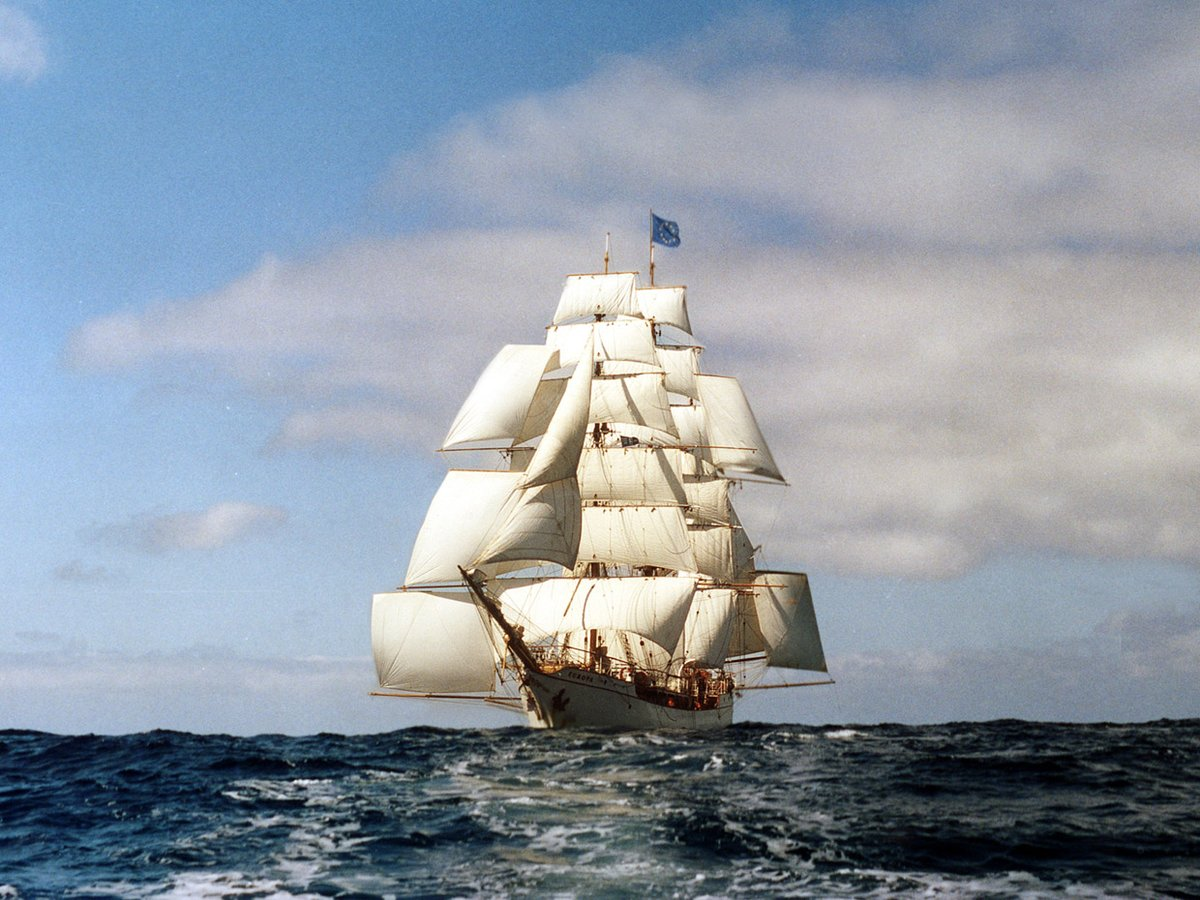
\includegraphics[width=0.5\textwidth]{images/foto}
	\caption{A Hold meghódítása}
	\label{fig:foto}
\end{figure}

\begin{multicols}{2}
	A repüléseket egy speciális űrhajórendszerrel hajtották végre, amely az Apollo típusú űrhajóból és a holdra szállás kulcsának számító holdkompból állt, hordozóeszközként pedig szintén speciálisan a feladathoz tervezett Saturn V és Saturn IB rakétákat használtak. A program hardverét később sikerrel alkalmazták más űrkutatási programokban is, így a Skylab-programban és az Szojuz–Apollo repülésen is.
	
	A program 1972-ben fejeződött be, azóta egyetlen embert szállító űrhajó sem hagyta el az alacsony Föld körüli pályát. Az űrhajósok által visszahozott kőzetminták és a kihelyezett műszerek mérései forradalmi változásokat hoztak a Naprendszer történetének, kialakulásának megismerésében, a Föld-Hold rendszer fejlődéstörténetének ismereteiben.
\end{multicols}

A repüléseket egy speciális űrhajórendszerrel hajtották végre, amely az Apollo típusú űrhajóból és a holdra szállás kulcsának számító holdkompból állt, hordozóeszközként pedig szintén speciálisan a feladathoz tervezett Saturn V és Saturn IB rakétákat használtak. A program hardverét később sikerrel alkalmazták más űrkutatási programokban is, így a Skylab-programban és az Szojuz–Apollo repülésen is.

A program 1972-ben fejeződött be, azóta egyetlen embert szállító űrhajó sem hagyta el az alacsony Föld körüli pályát. Az űrhajósok által visszahozott kőzetminták és a kihelyezett műszerek mérései forradalmi változásokat hoztak a Naprendszer történetének, kialakulásának megismerésében, a Föld-Hold rendszer fejlődéstörténetének ismereteiben.

Az Egyesült Államok az Apollo-programra több mint 19,5 milliárd dollárt költött.

\section{Előzmények}

\subsection{Korai elképzelések}
% definiáltunk egy többhasábos parancsot, ami elválasztó vonalat tesz az oszlopok közé
\begin{multicolss}{3} 
	Röviddel Konsztantyin Ciolkovszkij rakétaelvet megalkotó munkáinak publikálása után megjelentek az első elképzelések a világűr, azon belül pedig a legkézenfekvőbb cél, a Hold elérésére. Ezek közül a később legértékesebbnek bizonyult elképzelés Jurij Kondratyuk munkája volt, aki az 
	\columnbreak % hasábtörés
	anyaűrhajó/holdkomp rendszerű holdra szállás elméleti alapjait fektette le. Fantasztikus elképzelésekben később sem volt hiány, ilyen volt a három legkomplexebb ismeretekkel rendelkező tudós, Wernher von Braun rakétamérnök, Fred Whiplle és Willy Ley csillagászok publikációja a Holdutazás megvalósításáról a Colier's magazinban,[5] ami utópiának tűnt az 1950-es évek elején. Ebben az elképzelésben 15 űrhajós utazott volna, három óriási űrhajóval, amelyeket Föld körüli pályán szereltek volna össze, majd töltöttek volna fel üzemanyaggal. A háromból az egyik teherűrhajó lett volna, aminek célja pusztán a visszaútra szükséges üzemanyag szállítása lett volna. A leszállás után 6 hétig lettek volna az űrhajósok a Hold felszínén, napfelkeltétől kezdve egészen a következő – négy földi hétig tartó – nappal végéig. A kiürült üzemanyagtartályok hengereit lakómodulokká lehetett volna alakítani, egyfajta Hold-bázist létrehozva. Az építkezést daruk, és egy tíztonnás traktor (amit a későbbi felfedező utak járműveként is lehetett volna használni) könnyítette volna meg. Ennek az elképzelésnek a megvalósításához több száz tonna anyagot kellett volna megmozgatni, mindezt abban az időben, amikor az 1 tonnás Mercury-űrkabint sem tudták biztonságosan Föld körüli pályára állítani.[6]
\end{multicolss}


\begin{table}[H]
	\centering
	\begin{tabular}{ccc}
		\toprule
		Repülés & Dátum & Időtartam \\
		\midrule
		Apollo-7 & 1968 október 11. & 11 nap \\
		Apollo-8 & 1968 november 21. & 7 nap \\
		Apollo-9 & 1969 március 3 &  10 nap \\
		\bottomrule
	\end{tabular}
	\caption{Repülések}
	\label{tab:repulesek}
\end{table}

\subsection{Közvetlen előzmények}

\subsubsection{„Szputnyik-krízis”}

A hidegháború két egymással vetekedő nagyhatalma az 1950-es évek végén, a nemzetközi geofizikai év tudományos kísérlet- és rendezvénysorozatában találta meg azt az új területet, ahol kiterjeszthetik a technológiai versengésüket: az Egyesült Államok és a Szovjetunió egyaránt a világűrbe kívánta juttatni a maga űreszközét. A cél a másik fél fölötti technológiai fennhatóság bizonyítása volt. A versenyt a szovjetek nyerték, amikor 1957. október 4-én sikerrel juttatták az űrbe az addig titokban fejlesztett rakétájukkal a Szputnyik–1-et. Az USA-ban ezt szinte háborús hadüzenetként értelmezték (a szovjetek érdemi üzenete a műhold Föld körüli pályára állításával az volt: ha körbe tudunk juttatni a Földön egy tárgyat, akkor a Föld bármely pontját elérhetjük, bármely pontját képesek vagyunk bombázni).

Az USA vezetése elfogadta a szovjet kihívást és koncentrált erőfeszítést tett az űrteljesítmények területén az ellenfél előnyének behozására. E cél elérésére létrehozták a NASA-t, amely az összes korábban létrehozott repülési és űrhajózási kísérleti műhelyt vonta egy szervezetbe, hogy az erőket egyesítve minél hatékonyabban érjék el a kitűzött célt. 

\section{TikZ rajz}

Egy példa egy TikZ-ben rajzolt folyamat ábrára:

\begin{figure}[H]
	\centering
	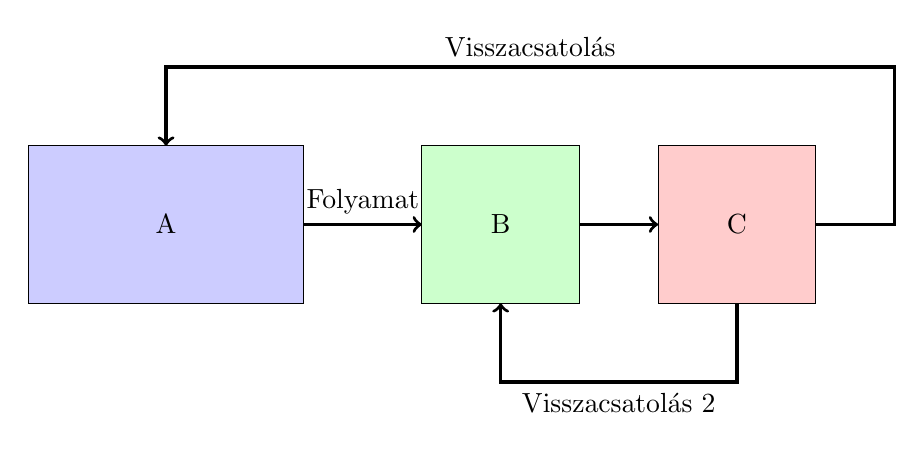
\begin{tikzpicture}
		% Solar panel
		\draw[fill=blue!20] (0,0) rectangle (3.5,2);
		\node at (1.75,1) {A};
		
		% Arrow
		\draw[->, very thick] (3.5,1) -- (5,1) node[midway, above] {Folyamat};
		
		% Battery
		\draw[fill=green!20] (5,0) rectangle (7,2);
		\node at (6,1) {B};
		
		% Arrow
		\draw[->, very thick] (7,1) -- (8,1);
		
		% Motor
		\draw[fill=red!20] (8,0) rectangle (10,2);
		\node at (9,1) {C};
		
		\draw[->, very thick] (10,1) -- (11,1) -- (11,3) -- (1.75,3)node[midway, above]{Visszacsatolás} -- (1.75,2) ;
		
		\draw[->, very thick] (9, 0) -- (9, -1) -- (6,-1)node[midway, below]{Visszacsatolás 2} -- (6,0);
		
	\end{tikzpicture}
	\caption{Rendszer block diagram}
	\label{fig:system}
\end{figure}

\section{Kapcsolási rajzok}

Kapcsolási rajzok CircuiTikZ-zel (európai konvenció szerint):

\begin{figure}[H]
	\centering
	\begin{minipage}[c]{0.4\textwidth}
		\centering
		\begin{circuitikz}[european]
			\draw (0,0) to[battery1, l=$V_s$] (0,3)
			to[R, l=$R_1$] (3,3)
			to[C, l=$C_1$] (3,0) -- (0,0);
		\end{circuitikz}
		\caption{Első ábra}
		\label{fig:elso}
	\end{minipage}\hfill\vrule\hfill
	\begin{minipage}[c]{0.55\textwidth}
		\centering
			\begin{tikzpicture}
			% Paths, nodes and wires:
			\node[op amp] at (6.833, 6.039){};
			\draw (4.25, 6.75) to[european resistor] (4.25, 8.75);
			\draw (4.25, 6.25) to[european resistor] (4.25, 4.25);
			\draw (4.25, 6.75) -| (4.25, 6.25);
			\draw (5.643, 6.529) -| (4.25, 6.5);
			\node[circ] at (4.25, 6.529){};
			\node[rground] at (4.25, 4){};
			\draw (5.25, 5.5) to[european voltage source] (5.25, 4);
			\draw (5.643, 5.549) -| (5.25, 5.5);
			\draw (4.25, 4.25) -| (4.25, 4);
			\node[rground] at (5.25, 4){};
			\draw (4.25, 8.75) -| (8.5, 6) |- (8.023, 6.039);
			\node[vcc] at (4.25, 9.25){};
			\draw (4.25, 9.25) -| (4.25, 8.75);
			\node[shape=rectangle, minimum width=0.715cm, minimum height=0.215cm](N1) at (4.625, 9.875){} node[anchor=center] at (N1.text){$U_{ki}$};
			\node[shape=rectangle, minimum width=0.715cm, minimum height=0.465cm](N2) at (6.125, 4.5){} node[anchor=center] at (N2.text){$U_{be}$};
			\draw[-latex] (5.75, 4) -- (5.75, 5.25);
			\node[circ] at (4.25, 8.75){};
		\end{tikzpicture}
		\caption{Második ábra}
		\label{fig:masodik}
	\end{minipage}
	\label{fig:circuit}
\end{figure}

Azt javaslom, hogy amennyiben kapcsolási rajzot szeretnél beilleszteni a dokumentációba és azt nem a schematicból fotózod ki, azaz megrajzolnád a dokumentációhoz, akkor ne manuálisan kódoljad le TikZ, vagy CircuiTikZ-ben, hanem használj egy olnile toolt, majd az ott kapott forráskódot másoljad be a forrásfile-ba: \underline{\url{https://www.circuit2tikz.tf.fau.de/designer/}}
